\section{Algorytm Chudnowsky'ch}

Algorytm zaproponowany przez braci Chudnowsky opiera się na 17 wzorach na $\frac1\pi$ opracowanych przez Srinivasa Ramanujan\cite{review}:
$${\frac {1}{\pi }}={\frac {1}{426880{\sqrt {10005}}}}\sum _{k=0}^{\infty }{\frac {(6k)!(13591409+545140134k)}{(3k)!(k!)^{3}(-640320)^{3k}}}.$$
Z tego można uzyskać $\pi$ wprost w formie wzoru:
$$\pi=C\Big(\sum\limits_{q=0}^\infty{M_q\cdot L_q\over X_q}\Big)^{-1},$$
gdzie 
$$
\begin{cases}
    C=426880\sqrt{10005}\\
    L_{q+1}=L_q+545140134 \quad L_0=13591409  \\
    X_{q+1}=X_q\cdot(-262537412640768000)\quad X_0=1\\
    K_{q+1}=K_q+12\quad K_0=-6\\
    M_{q+1}=M_{q}\cdot \left({\frac {K_{q+1}^{3}-16K_{q+1}}{\left(q+1\right)^{3}}}\right)\quad M_{0}=1.
\end{cases}
$$
Aby wyprowadzić ten wzór, jak i inne podane przez Ramanujana, potrzebna jest znajomość między innymi teorii funkcji eliptycznych\cite{review}. Z tego też względu w tym reporcie nie podejmiemy się uzasadniania poprawności wyżej podanego wzoru. Dla zainteresowanych polecamy lekturę "Collected Papers of Srinivasa Ramanujan"\cite{ramanujan}.

\begin{figure}[!h]
    \centering
    \renewcommand{\figurename}{Wykres}
    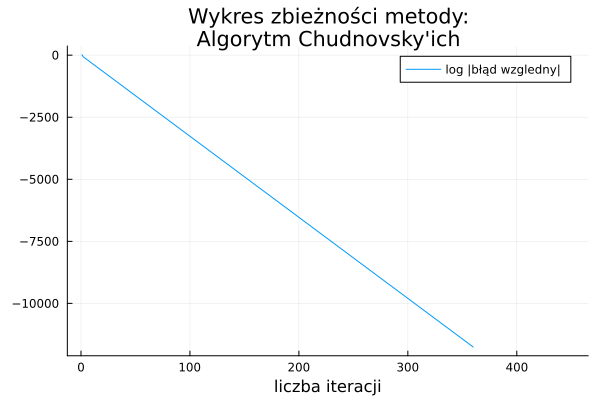
\includegraphics[width=0.7\textwidth]{../prog/chudnowsky_log_error.png}
    \caption{Wykres logarytmu dziesiętnego z błędu względnego dla przybliżenia $\pi$ za pomocą algorytmu braci Chudnowsky'ch.}
    \label{chudnowsky-error}
\end{figure}

\begin{figure}[!h]
    \centering
    \renewcommand{\figurename}{Wykres}
    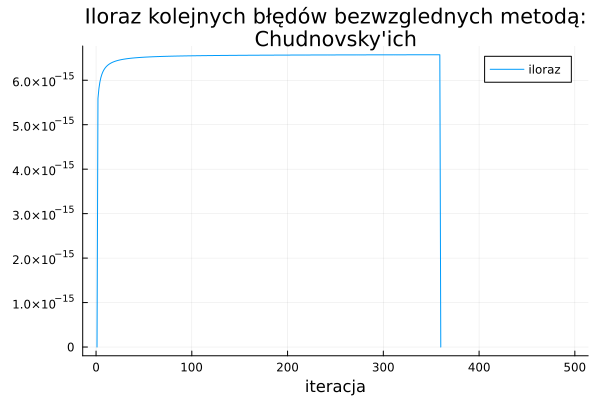
\includegraphics[width=0.7\textwidth]{../prog/chudnowsky_error_ratio.png}
    \caption{Wykres ilorazu błędów względnych wyrazu $n+1$ i $n$ dla algorytmu Chudowsky'ch.}
    \label{chudnowsky-convergence}
\end{figure}

\subsection{Wyniki}

Logarytm z błędu względnego algorytmu Chudnowsky'ch dla pierwszych 400 iteracji został zaprezentowany na Wykresie~\ref{chudnowsky-error}. Już dla 359 iteracji błąd bezwzględny jest równy 0. Każe to sugerować, że to właśnie ta metoda została użyta jako implementacja funkcji \verb+pi()+ w języku \verb+Julia+. Dlatego od 359 iteracji nie ma zaznaczonej wartości $\log_{10}$ od błędu względnego. Powoduje to anomalie widoczne na wykresach.

Eksperymentalne wyznaczanie zbieżności metody Chudnowsky'ch sugeruje zbieżność liniowa, tak jak na Wykresie~\ref{chudnowsky-convergence}.. Nietypowe załamanie w okolicach 359 iteracji jest spowodowane zerową wartością błędu bezwzględnego w tym miejscu. Z pozostałej części wykresu możemy wydedukować, że
$$\lim_{k\to\infty}{{|x_{k+1}-\pi|\over |x_k-\pi|}}\approx 6.5\cdot 10^{-15},$$
gdzie $x_k$ to oszacowanie $\pi$ uzyskane w $k$-tej iteracji.